\section{Code Readability vs.~Speed of Execution}\label{code-readability-vs.speed-of-execution}

Programmers throughout time have had to deal with speed of code execution and it's an ongoing concern.~ However, compilers are pretty smart these days and, often, can produce speedier code for the hardware platform than the programmer can when he or she uses ``speed up'' tips.~ The EnergyPlus development team would rather the code be more ``readable'' to all than to try to outwit the compilers for every platform.~ First and foremost, the code is the true document of what EnergyPlus does -- other documents will try to explain algorithms and such but must really take a back seat to the code itself.

However, many people may read the code -- as developers, we should try to make it as readable at first glance as possible.~ For a true example from the code and a general indication of preferred style, take the case of the zone temperature update equation.~ In the \href{file:///E:/Docs4PDFs/EngineeringReference.pdf}{Engineering Reference} document, the form is recognizable and usual:

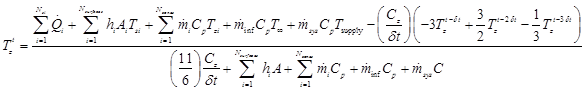
\includegraphics{media/image001.png}And, this equation appears in the code (ZoneTempPredictorCorrector Module), as:

ZT(ZoneNum) = (CoefSumhat +~~ CoefAirrat*(3.0*ZTM1(ZoneNum) - (3.0/2.0)*ZTM2(ZoneNum) \&

~~~~~~~~~~~~~~~~~~~~~~~~~~~~~~~~~~~~~~~~~~~~~ + (1./3.)* ZTM3(ZoneNum))) \&

~~~~~~~~~~~~~~~~~~~~~~~~~~~~ / ((11.0/6.0)*CoefAirrat+CoefSumha)

Somewhat abbreviated here due to lack of page width but still recognizable from the original.~ A better version would actually be:

ZT(ZoneNum) = (CoefSumhat -~~ CoefAirrat*(-3.0*ZTM1(ZoneNum) + (3.0/2.0)*ZTM2(ZoneNum) \&

~~~~~~~~~~~~~~~~~~~~~~~~~~~~~~~~~~~~~~~~~~~~~ - (1./3.)* ZTM3(ZoneNum))) \&

~~~~~~~~~~~~~~~~~~~~~~~~~~~~ / ((11.0/6.0)*CoefAirrat+CoefSumha)

Whereas the natural tendency of programming would lead to the less readable:

ZT(ZoneNum) = (CoefSumhat + CoefAirrat*(3.0*ZTM1(ZoneNum) -- 1.5*ZTM2(ZoneNum) + .333333* ZTM3(ZoneNum))) \&

~~~~~~~~~~ / (1.83333*CoefAirrat+CoefSumha)

The final version is a correct translation (more or less) from the Engineering/usual representation but much harder to look at in code and realize what is being represented.

\subsection{Speed of Execution}\label{speed-of-execution}

\textbf{A critical consideration in speed of execution is character string comparisons.}~ These are typically quite slow and should not be used in the core routines (i.e.~those that are executed every zone or hvac time step). An alternative to string comparisons is to define module-level integer parameters, equate a string to a parameter during the initial subroutine call (e.g.~GetInput), and then do integer comparisons through the remainder of the calls to the module.~ Doing this does not deter readability, yet assists in reducing execution time.

For example, in the module shown previously (Module Fans), the parameters for fan types are set as Integers:

~ !MODULE PARAMETER DEFINITIONS

INTEGER, PARAMETER :: FanType\_SimpleConstVolume = 1

INTEGER, PARAMETER :: FanType\_SimpleVAV~~~~~~~~ = 2

INTEGER, PARAMETER :: FanType\_SimpleOnOff~~~~~~ = 3

INTEGER, PARAMETER :: FanType\_ZoneExhaust~~~~~~ = 4

During the GetInput, string types are shown (this is getting these objects):

~~~~~~~ CALL GetObjectItem(`FAN:SIMPLE:CONSTVOLUME',~ \&

~~~~~~~~~~~~~~~~~~~~~~~~~~ SimpFanNum,AlphArray, \&

~~~~~~~~~~~~~~~~~~~~~~~~ ~~NumAlphas,NumArray,NumNums,IOSTAT)

~~~~~~~ . . .

~~~~~~~ Fan(FanNum)\%FanName = AlphArray(1)

~~~~~~~ Fan(FanNum)\%FanType = `SIMPLE'

~~~~~~~ . . .

~~~~~~~ Fan(FanNum)\%Control = `CONSTVOLUME'

~~~~~~~ Fan(FanNum)\%FanType\_Num = FanType\_SimpleConstVolume

Then, during the simulation the integer parameters are used:

~ ! Calculate the Correct Fan Model with the current FanNum

~ IF (Fan(FanNum)\%FanType\_Num = = FanType\_SimpleConstVolume) THEN

~~~ Call SimSimpleFan(FanNum)

~ Else IF (Fan(FanNum)\%FanType\_Num = = FanType\_SimpleVAV) THEN

~~~ Call SimVariableVolumeFan(FanNum)

~ Else If (Fan(FanNum)\%FanType\_Num = = FanType\_SimpleOnOff) THEN

~~~ Call SimOnOffFan(FanNum)

~ Else If (Fan(FanNum)\%FanType\_Num = = FanType\_ZoneExhaust) THEN

~~~ Call SimZoneExhaustFan(FanNum)

~ End If

This does not detract from code readability at all but execution is much speedier with this versus the string comparisons.
